% Primarily this section should be about scientific methods and theories you need to evaluate/compare/invent to solve your problems from 1.3.
% In some cases it may be ok to describe different technologies, but the purpose is to describe something and then draw a conclusion from that.
% Example, if you decide to discuss different databases, it may be for the purpose of selecting the best type for your implementation later on (based on for example data representation, scalability, speed, etc.).
% Optimally the problems in 1.3 are not solved by anyone else yet, in which case this section needs to describe how to solve them (new algorithms, mathematical approaches, etc.).
 
% This section can have a lot of subsections (3.1, 3.2, 3.3, etc).


% TODO: Explain DWARF Sections
The \gls{DWARF} format is divided into sections in the object file which all contain specific information, these sections use offsets to point to information in another section, see figure \ref{fig:dwarfsections}.
All of the sections can be different from depending on \gls{DWARF} versions and some doesn't exist in the older versions.
Thus these explanations only apply to \gls{DWARF} version $4$ and some of the older versions, checkout Appendix F in \cite{dwarf} for more information.


\begin{figure}[h]
    \centering
    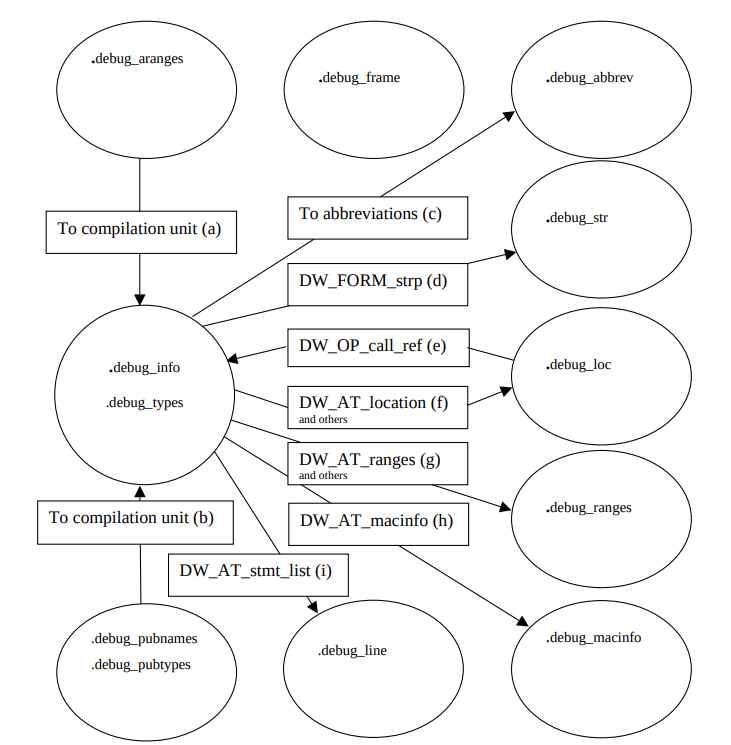
\includegraphics[width=1.0\textwidth]{dwarf-sections.png}
    \label{fig:dwarfsections}
\end{figure}


Going in alphabetical order the first \gls{DWARF} section is called \emph{.debug\_abbrev}.
This section contain all of the abbreviation tables which can be used to find a specific die using the abbreviation.
These table entries contain information about the die tag, attributes and if it has children.
The library \emph{gimli-rs} simplifies the process of using this table and thus removes the need to know the detail of how to read it, but checkout section 7.5.3 in \cite{dwarf} to know more.


The \gls{DWARF} section \emph{\.debug\_aranges} is used to lookup which machine address corresponds to which compilations unit.
This address information is stored in ranges where a compilation unit can have multiple ranges.
These ranges consists of a start address followed by length.
Thus to lookup the user only needs to check if the search address is between the start address and the start address plus the length.
To read more about this section checkout section 6.1.2 in \cite{dwarf}.


In the \gls{DWARF} section \emph{.debug\_frame} the information needed to virtually unwind the call stack is kept.
Unwinding the call stack is complex and is hardware specific but the \emph{gimli-rs} library simplifies the process a lot.
This section is completely self-contained and is made up of two structures called \acrfull{cie} and \acrfull{fde}.
To learn more of this section checkout section 6.4.1 in \cite{dwarf}


Information about the source code are store in \glspl{die} which are low-level representation of the source code.
These have a tag that describes what it represents, an example tag is \emph{DW\_TAG\_variable} which means that the \gls{die} represents a variable from the source code.
All \glspl{die} are stored in \gls{tree} structure that represents a compilation unit or a partial one.
These \gls{tree} structures are structure like the source program and makes it possible to relate the source code to the machine code.
The section \emph{.debug\_info} contains a number of units that all have one of these \gls{die} \glspl{tree} and some more important debug information.
Thus this is one of the most important sections in \gls{DWARF} because it is used to understand the relation ship between the source code and the machine code.


The \gls{DWARF} section \emph{.debug\_line} holds the needed information to find the machine addresses that is generated from a certain line and column in the source file.
It is also used to store the source director, file name, line number and column.
Then the \glspl{die} will store pointers to the source location information in the section \emph{.debug\_line} enabling the debugger to know the source location of a \gls{die}.
The section 6.2 in \cite{dwarf} explains in more detail how this information is stored in the \emph{.debug\_line} section.


The location of the variables values are stored in location lists, each entry in the list holds a number of operation that can be used to calculate the location of the value.
All of the location lists are stored in the section \emph{.debug\_loc} and are pointed to by \glspl{die} in the \emph{.debug\_info} section.
The pointers are most commonly found in the attribute \emph{DW\_AT\_location} which most dies representing variables have.
The relation between these sections can be seen in the figure \ref{fig:dwarfsections}.


In the section \emph{.debug\_macinfo} the macro information is stored, it is stored in entries that each represents the macro after it has been expanded by the compiler.
These entries are also pointer to by \glspl{die} in the \emph{.debug\_info} section and those pointers can be found in the attribute \emph{DW\_AT\_macinfo}.
This section is a little complex thus to learn more about it read section 6.3 in \cite{dwarf}.


There are two sections for looking up compilation units by name.
The first one is \emph{.debug\_pubnames} which is for finding functions and objects.
And the other one is for finding types, this section is called \emph{.debug\_pubtypes}.
Both of these work in the same way and are fairly simple to understand, checkout section 6.1.1 in \cite{dwarf} for more information.


\Glspl{die} that have a set of addresses that are non-contiguous will have offset in to the section \emph{.debug\_ranges} instead of having a address range.
This offset points to the start of a range list that contain range entries which are used to know for which addresses the \gls{die} is used in the program.
Checkout section 2.17 in \cite{dwarf} to learn more about code addresses and ranges.


The section \emph{.debug\_str} is used for storing all the strings that is in the debug information.
An example of these strings are the names of the functions and variables, these string are found using the offset in the attribute \emph{DW\_AT\_name}.
The attribute is found in the function and variable dies and the offset is in the form of \emph{DW\_FROM\_strp}.


The last section is \emph{.debug\_type} it is very similar to section \emph{.debug\_info} in that it is also made up of units with each a \gls{tree} of \glspl{die}.
The difference is that the \glspl{die} are a low-level representation of the types in the source code instead of a representation of the source program.

